\documentclass[12pt]{article}

\title{Real dimension in the Newtonian simulation of disk-like pressure-free systems}
\author{S. Halayka\footnote{sjhalayka@gmail.com}}
\date{\today\;\currenttime}

\usepackage{datetime}
\usepackage{listings}
\usepackage{cite}
\usepackage{xcolor}
\usepackage{graphicx}
\usepackage{setspace}
\usepackage{amsmath}
\usepackage{url}
\usepackage[margin=0.8in]{geometry}
\usepackage{listings}


\usepackage{xcolor}
\lstset { %
    language=C++,
    backgroundcolor=\color{black!5}, % set backgroundcolor
    basicstyle=\footnotesize,% basic font setting
    showstringspaces=false,
}


%\doublespace

%\usepackage[]{lineno}
%\linenumbers


\begin{document}



 
\maketitle

\begin{abstract}
Abstract...
\end{abstract}






\section{Brute force: field line intersection density gradient}
Regarding the holographic principle, where $n$ is the gravitational field line count, and $A_s$ is the Schwarzschild black hole event horizon area:
\begin{equation}
n = \frac{A_s k c^3}{ 4 G \hbar \log 2},
\end{equation}
the Schwarzschild radius is:
\begin{equation}
r_s = \sqrt{\frac{A_s}{4 \pi}} = \sqrt{\frac{n G \hbar \log 2}{k c^3 \pi}},
\end{equation}
and the mass is:
\begin{equation}
M = \frac{c^2 r_s}{2 G} = \sqrt{\frac{n c \hbar \log 2}{4 G k \pi}}. 
\end{equation}

Where $R$ is some far distance from the centre of the gravitating body (e.g, $R \gg r_s$), $\beta$ is the get intersecting line length function, and $\epsilon$ is some small value (e.g $10^{-5}$), the gradient is:
\begin{equation}
\gamma = \frac{\beta(R + \epsilon) - \beta(R)}{\epsilon}.
\end{equation}
The gradient strength is:
\begin{equation}
g = -\gamma \pi = \frac{n}{2 R^3}.
\end{equation}
The Newtonian acceleration $a_{\textit{Newton}}$ is:
\begin{equation}
a_{\textit{Newton}} = \frac{v_{\textit{Newton}}^2}{R} = \sqrt{\frac{g G c \hbar \log 2}{2 R^2 k \pi}}.
\end{equation}

The Newtonian acceleration $a_{\textit{flat}}$ for a flat rotation curve is:
\begin{equation}
a_{\textit{flat}} = \frac{v_{\textit{flat}}^2}{R} = \frac{g R c \hbar \log 2}{2 k \pi M}.
\end{equation}

The ratio of the acceleration is
\begin{equation}
\frac{a_{\textit{flat}}}{a_{\textit{Newton}}} = R^{d}, 
\end{equation}
where $d = 3 - D$ stands for disk-like, and the dimension of the gravitation field is:
\begin{equation}
D = 3 - \frac{\log \frac{a_{\textit{flat}}}{a_{\textit{Newton}}}}{\log R} = 3 - \frac{\log \frac{v_{\textit{flat}}^2}{v_{\textit{Newton}}^2}}{\log R}.
\end{equation}




\begin{figure} 
\centering
\label{fig1}
  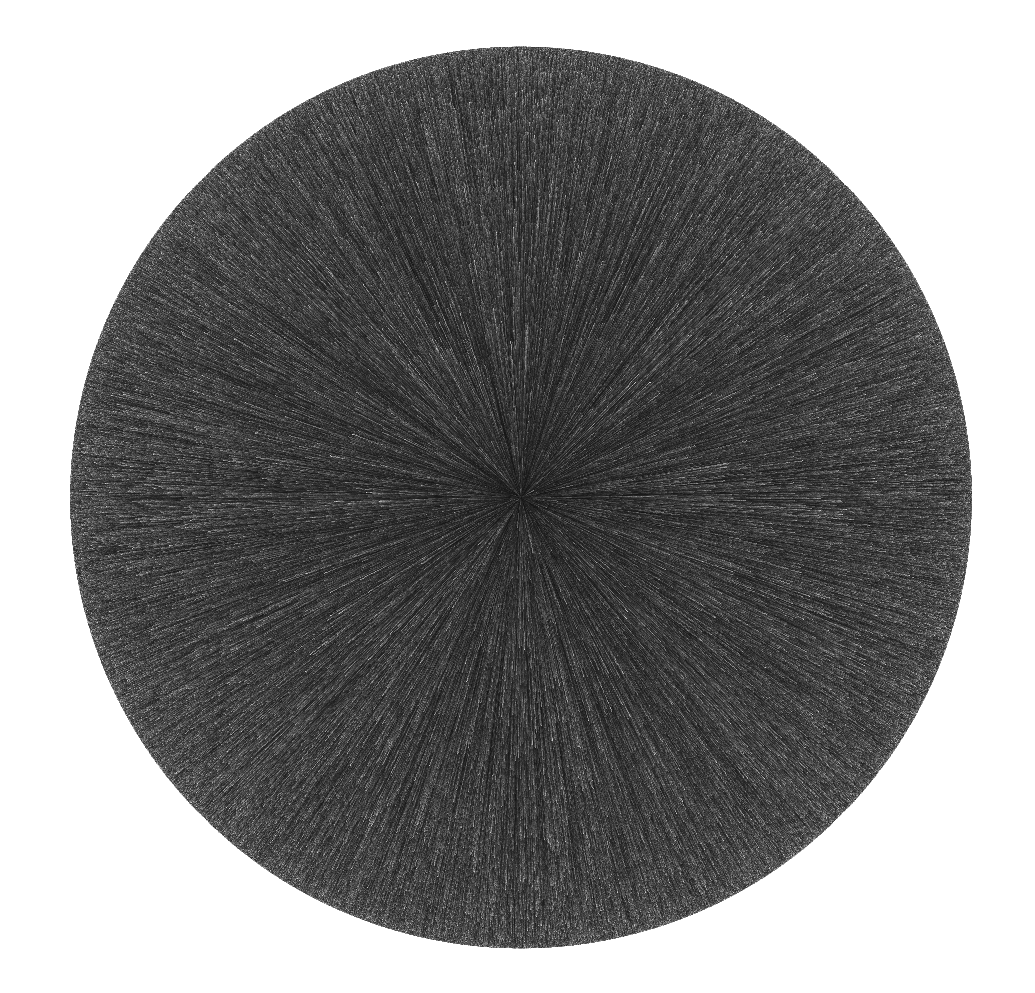
\includegraphics[width = 3 in]{3.png}
  \caption{
Where $D = 3$.
The normals are isotropic.
}
\end{figure}

\begin{figure} 
\centering
\label{fig2}
  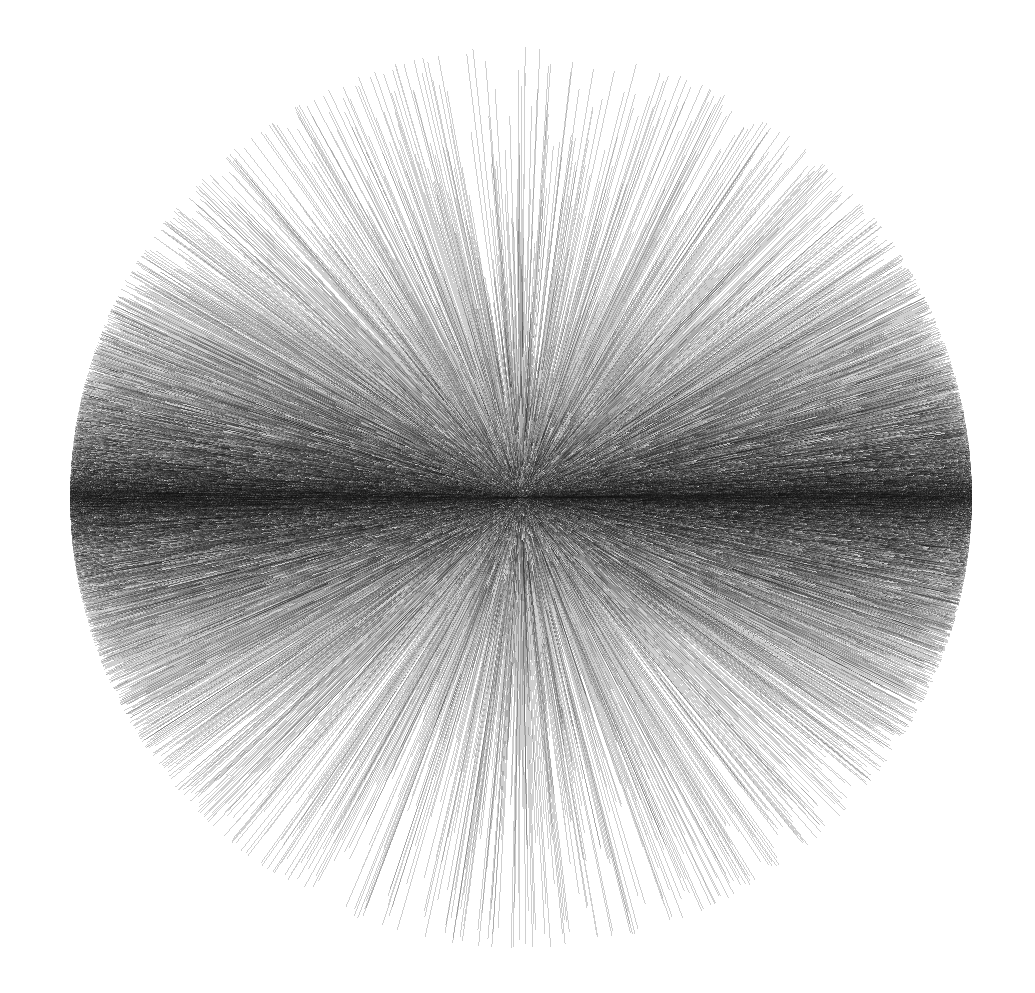
\includegraphics[width = 3 in]{2.1.png}
  \caption{
Where $D = 2.1$.
The normals are increasingly anisotropic.
}
\end{figure}

\begin{figure} 
\centering
\label{fig3}
  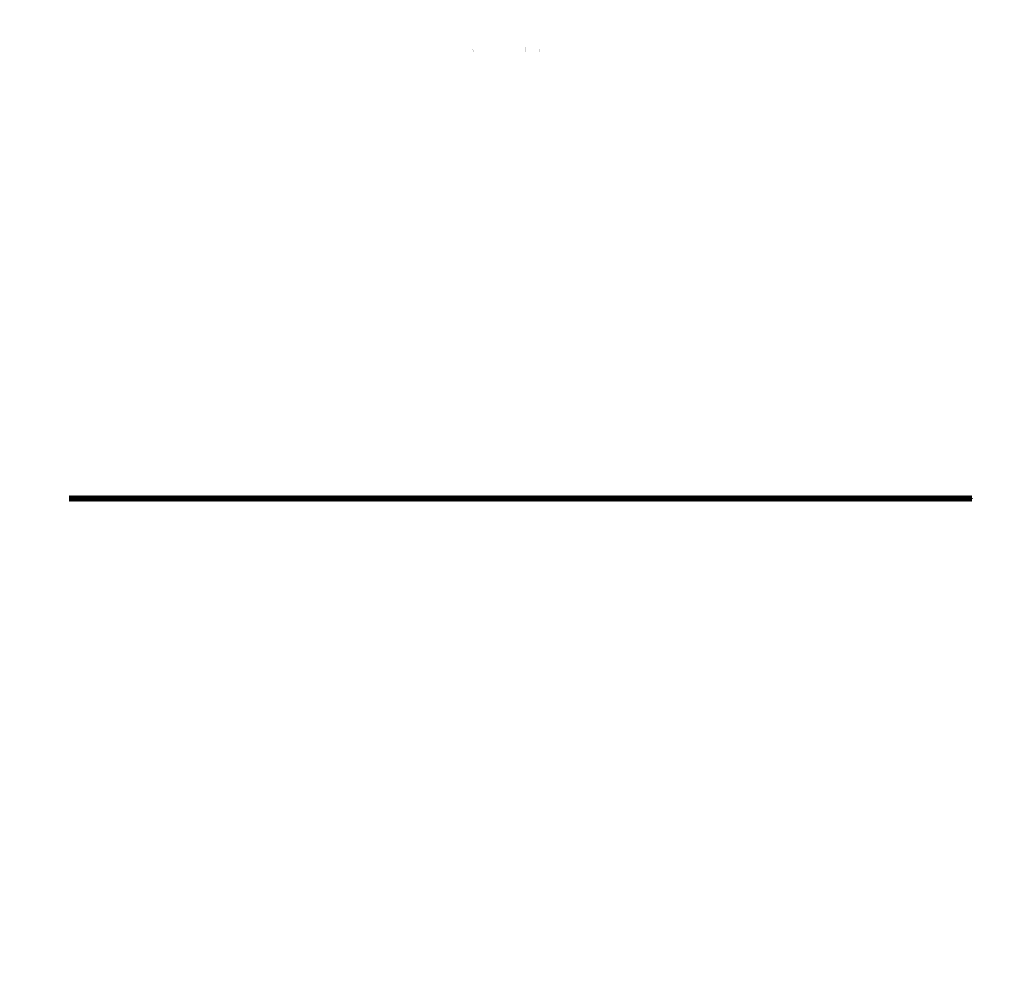
\includegraphics[width = 3 in]{2.001.png}
  \caption{
Where $D = 2.001$.
The normals are anisotropic.
}
\end{figure}


\begin{figure} 
\centering
\label{fig4}
  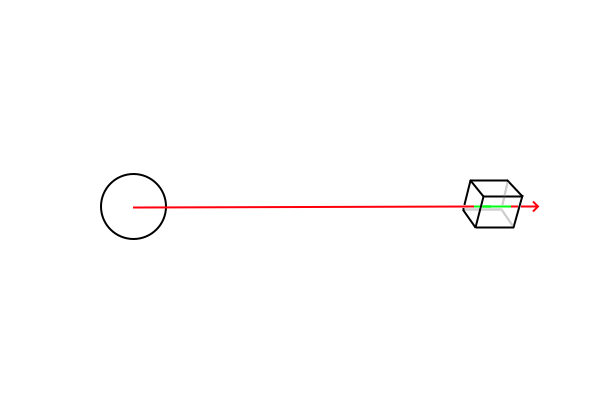
\includegraphics[width = 5 in]{AABB.png}
  \caption{
Where $D = 3$.
This figure shows an axis-aligned bounding box and an isotropic emitter, looking from above.
The bounding box is filled with the intersecting line segments.
}
\end{figure}



\begin{lstlisting}
#include <cmath>
#include <iostream>
using namespace std;

const double G = 6.67430e-11;
const double c = 299792458;
const double c2 = c * c;
const double c3 = c * c * c;
const double pi = 4.0 * atan(1.0);
const double h = 6.62607015e-34;
const double hbar = h / (2.0 * pi);
const double k = 1.380649e-23;

int main(void)
{
	double M = 1e41;

	double r_s = 2 * G * M / c2;
	double A_s = 4 * pi * r_s * r_s;
	double n = A_s * k * c3 / (4 * G * hbar * log(2.0));

	double R = 3e20;
	double g = n / (2 * R * R * R);

	double a_Newton = sqrt((g * G * c * hbar * log(2.0))/(2 * R*R * k * pi));
	double a_flat = pow(220000, 2.0) / R;

	double v_Newton = sqrt(a_Newton * R);
	double v_flat = 220000;

	double D = 3.0 - log(a_flat / a_Newton) / log(R);
	double D_ = 3.0 - log(pow(v_flat, 2.0) / pow(v_Newton, 2.0)) / log(R);

	cout << D << endl;
	cout << D_ << endl;

	return 0;
}
\end{lstlisting}

%\pagebreak







\begin{thebibliography}{9}

\bibitem{misner} Misner et al. Gravitation. (1970)

\bibitem{hooft} `t Hooft. Dimensional reduction in quantum gravity. (1993)
\bibitem{susskind} Susskind. The World as a Hologram. (1994)





%\bibitem{nasa} Williams. NASA Mercury Fact Sheet. (2024)



\end{thebibliography}














\end{document}









